%! Author = stefano
%! Date = 21-May-20

% Preamble
\documentclass[11pt]{article}
\title{Algoritmi Avanzati: Travelling Salesman Problem}
\author{Zanatta Stefano}

% Packages
\usepackage{amsmath}
\usepackage{graphicx}
\usepackage[utf8]{inputenc}
\usepackage{float}
\usepackage{natbib}

% Document
\begin{document}
\maketitle
\section{Implementazione}\label{sec:implementazione}
    Ho implementato, in Python, tre algoritmi per il Travelling Salesman Problem (TSP).
    \begin{itemize}
        \item Held\-Karp: l'implementazione è fedele all'algoritmo; ho dovuto aumentare il limite massimo di chiamate ricorsive (da $10^4$ a $10^6$);
        \item Random Insertion: composta da tre funzioni
            \begin{itemize}
                \item initialize: fase di inizializzazione, crea un circuito composto dal nodo zero e il più vicino a questo;
                \item random\_insert: metodo principale, comprende la fase di selezione (randomica, tra i nodi non visitati);
                \item insert: inserisce il nodo selezionato nel circuito;
            \end{itemize}
        \item mst\_tsp: algoritmo basato sul minimum spanning tree, in particolare con Prim; trova un minimum spanning tree, calcola la preorder list (cioè il circuito approssimato), aggiunge il nodo radice alla fine della lista, per chiudere il circuito e ritorna il suo peso.
    \end{itemize}
    Solo l'implementazione di Held-Karp è limitata nel tempo (180 secondi per file).
    Se viene raggiunto il tempo limite, vengono comunque fatte le chiamate ricorsive necessarie per avere un risultato differente da {$\infty$}.\\
    Il grafo è implementato tramite lista di adiacenza.
    Solo per l'algoritmo mst\_tsp, ho adattato la lista di adiacenza al codice del primo progetto, trasformandola in una istanza della classe classe Graph.\\
    Ho parallelizzato l'esecuzione degli algoritmi in due fasi: prima Held Karp, poi i restanti.
    In ogni fase, ogni input esegue in parallelo con gli altri.
    Ho fatto questa divisione per garantire più memoria e cpu a Held Karp.
\section{Risultati}\label{sec:risultati}
    L'algoritmo di Held-Karp richiede più tempo d'esecuzione rispetto alle euristiche e mst\_tsp.
    Se la taglia dell'input è sufficentemente piccola, il risultato è corretto. In caso contrario, raggiunge il limite di 3 minuti e ritorna un pessimo valore approssimato (errore del 30\% per grafi con 200 nodi, 96\% sul un grafo con 1000 nodi).
    Per poter eseguire tutte le chiamate ricorsive, ho dovuto aumentare considerevolmente il limite di chiamate ricorsive di Python (fino a $10^6$).\\
    L' euristica da risultati approsismati, con un errore fino  al 13\%.\\
    L'algoritmo basato sul mst ritorna risultati peggiori di Random Insertion, fino al 30\% di errore.
    Il migliore tra i tre algoritmi, rispetto all'errore e la velocità, è Random Insertion.\\
    A differenza di Held Karp, l'euristica e mst-tsp dipendono solo in parte dalla taglia dell'input: con pochi nodi i risultati sono generalmente buoni, ma con l'aumentare degli stessi, non c'è una crescita lineare dell'errore (per esempio, l'errore di ch150 è maggiore di dsj1000).
\begin{figure}[H]
    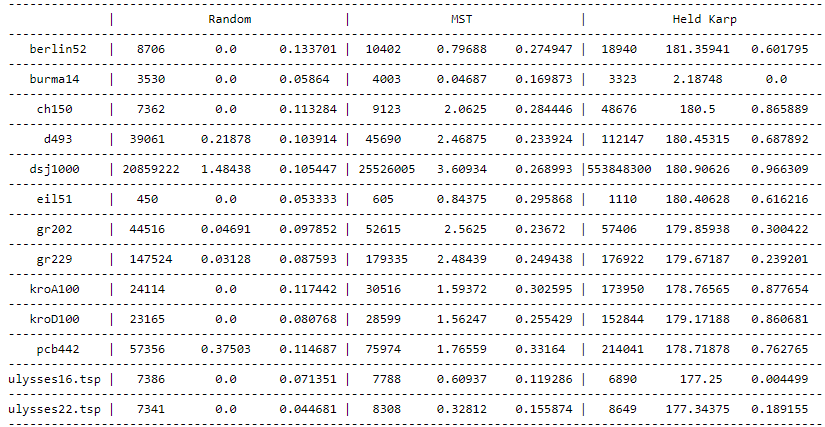
\includegraphics[width=1\textwidth]{table.PNG}
\end{figure}
\section{Considerazioni}\label{sec:considerazioni}
    Ho utilizzato una lista di adiacenza per rappresentare il grafo, perché più pratica rispetto ad una implementazione con una classe Python (come avevo fatto nel primo progetto).
    Ho riutilizzato del codice dal primo progetto (ridotto al minimo indispensabile) per calcolare il mst tramite Prim (nella cartella src.prim)\\
\end{document}